 %%%%%%%%%%%%%%%%%%%%%%%%%%%%%%%%%%%%%%%%%%%%%%%%%%%%%%%%%%%%%%%
%
% Welcome to Overleaf --- just edit your LaTeX on the left,
% and we'll compile it for you on the right. If you give 
% someone the link to this page, they can edit at the same
% time. See the help menu above for more info. Enjoy!
%
%%%%%%%%%%%%%%%%%%%%%%%%%%%%%%%%%%%%%%%%%%%%%%%%%%%%%%%%%%%%%%%

%  My thanks to Dana Ernst of Northern Arizona University for sharing 
%    his template with me. This is largely his work.
% --------------------------------------------------------------
% This is all preamble stuff that you don't have to worry about.
% Head down to where it says "Start here"
% --------------------------------------------------------------
 
\documentclass[12pt]{article}
 
\usepackage[margin=1in]{geometry} 
\usepackage{amsmath,amsthm,amssymb}
\usepackage{graphicx}
 
\newenvironment{theorem}[1][Theorem]{\begin{trivlist}
\item[\hskip \labelsep {\bfseries #1}]}{\end{trivlist}}


\begin{document}
 
% --------------------------------------------------------------
%                         Start here
% --------------------------------------------------------------
 
\title{Exterior Angles of a Triangle} % replace with an appropriate title, choose something shortish & descriptive
\author{Theron J Hitchman} % replace with your name, multiple authors go in alphabetical order by last name
 
\maketitle

{%
\centering
\textit{Communicated by: Mx. Thisis Great} % replace the name with the name of your referee(s)
\par
}
\hrule
\vspace{.2in}


For our third example paper, we rewrite Proposition I.16 from Euclid's \emph{Elements} in modern language.

\begin{theorem}[Euclid's Proposition I.16] Let $ABC$ be a triangle. Extend the side $BC$ to a ray $BD$ so that $C$ lies between $B$ and $D$. Then the exterior angle $ACD$ is greater than either of the remote interior angles $CAB$ or $ABC$.
\end{theorem}
 
\begin{proof}
First, we shall show that angle $ACD$ is greater than angle $CAB$.

Construct the midpoint $E$ of segment $AC$ by Euclid's Proposition I.10. Then we draw the ray $BE$ with initial point $B$ through $E$, and the circle with center $E$ which passes through $B$. This line and circle meet $B$, of course, and again at a point we will call $F$. Because they are both radii of the circle at $B$, $BE$ and $BF$ are congruent segments. Finally, we draw segment $CF$.

\begin{figure}[ht]
\centering
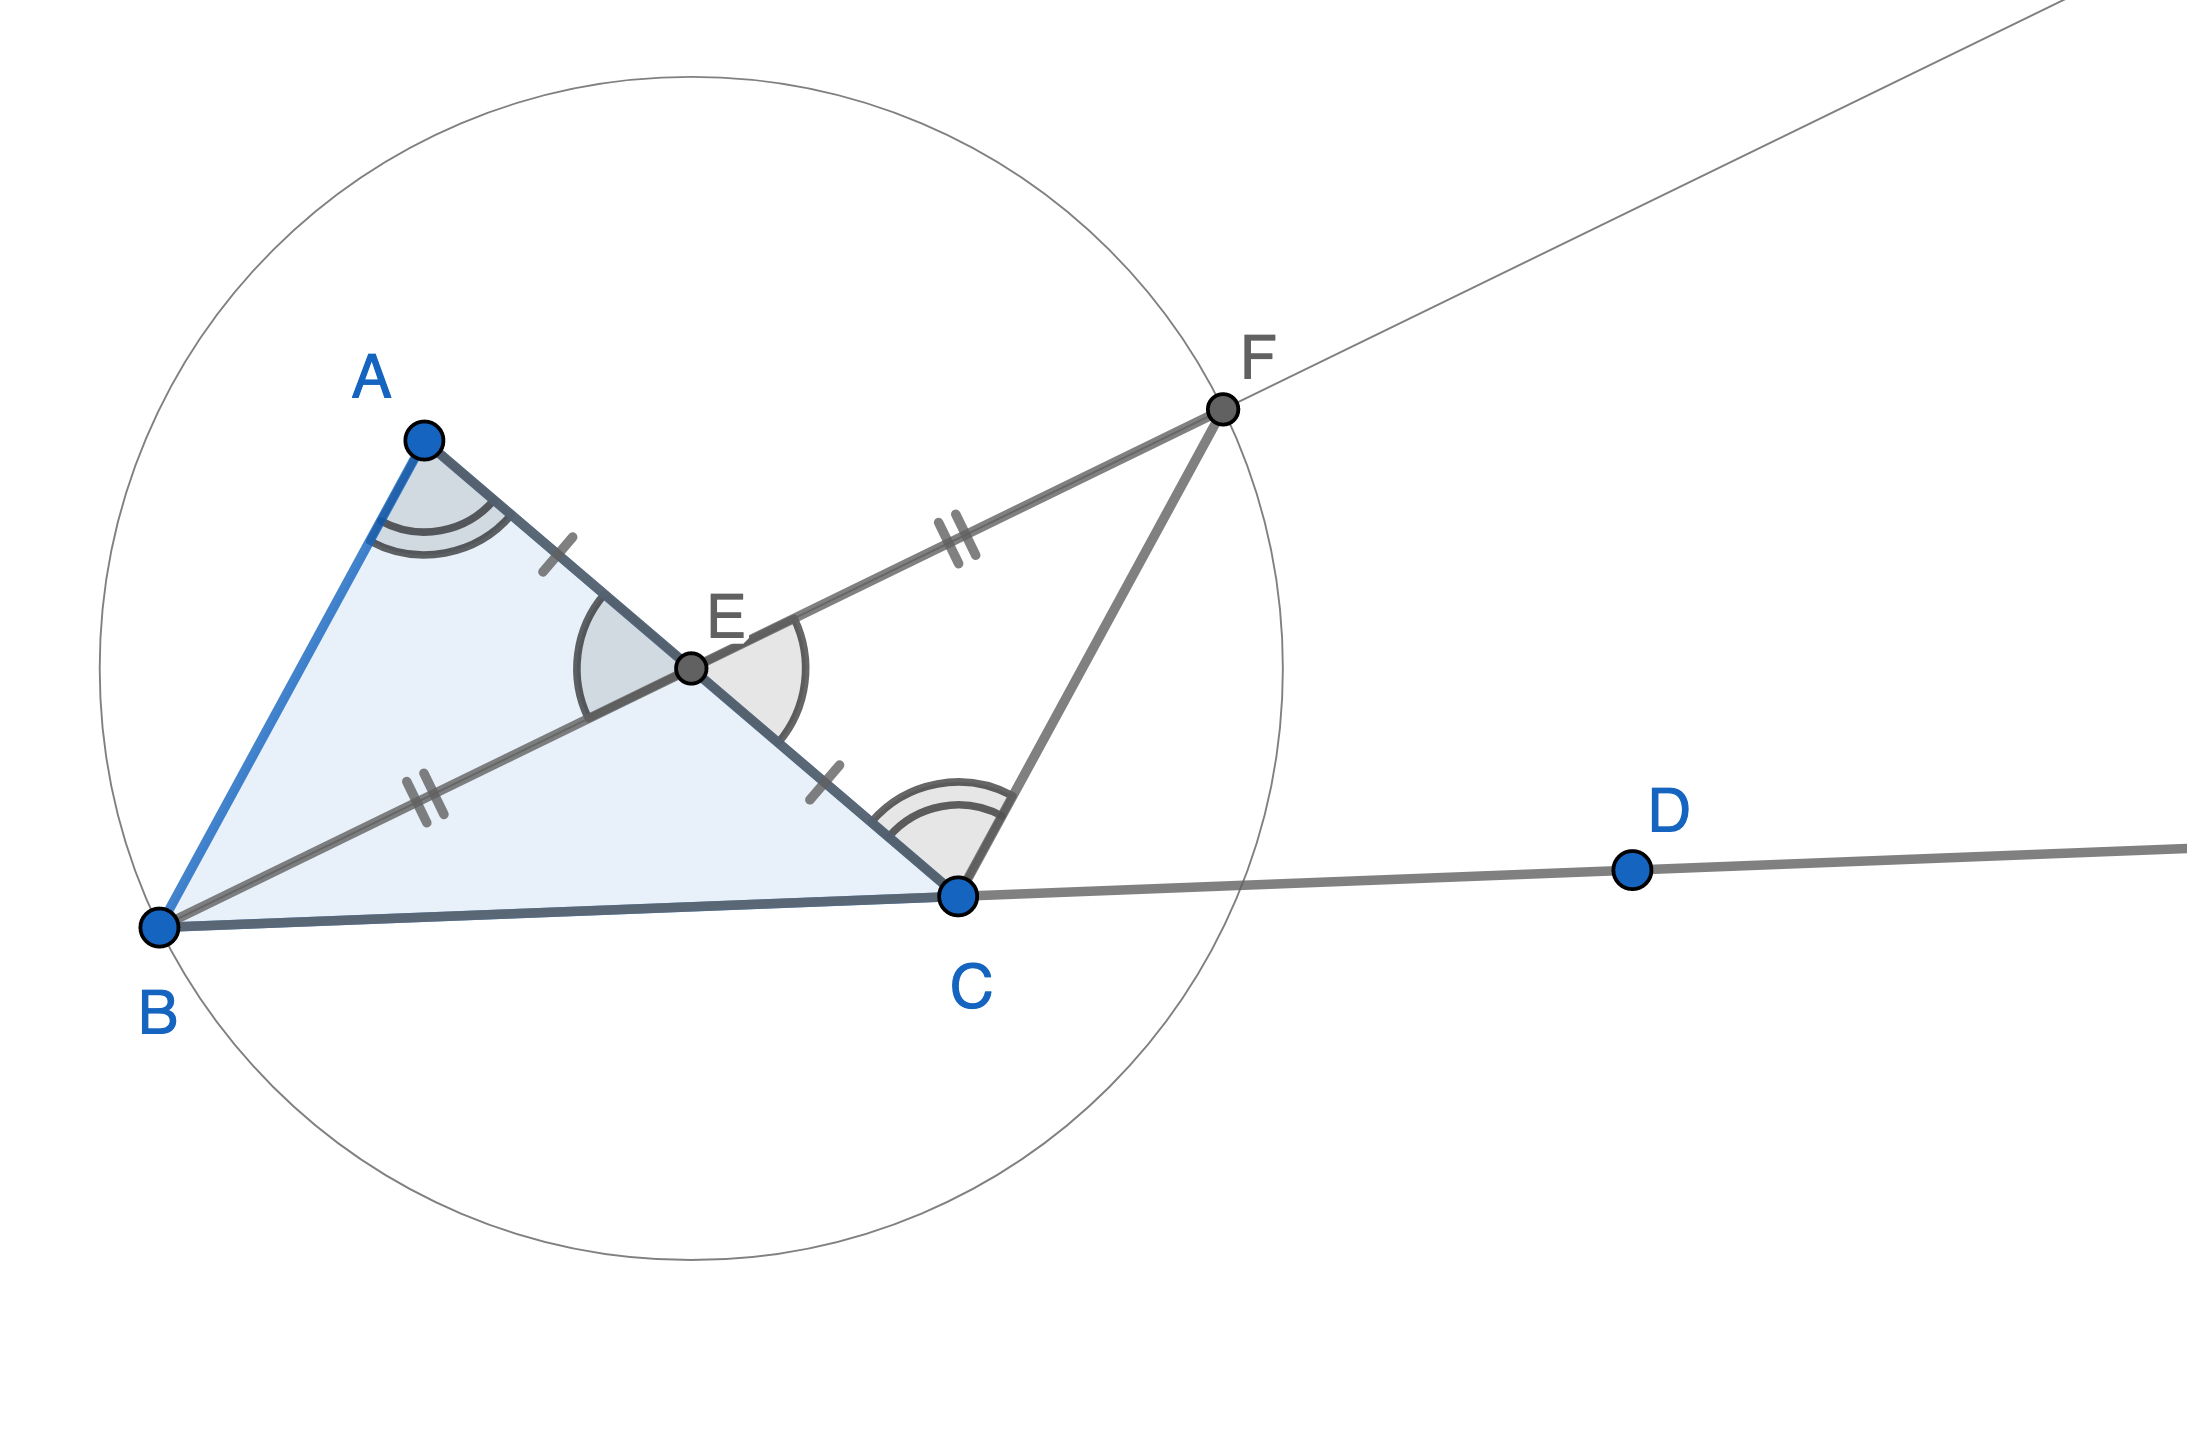
\includegraphics[width=.5\textwidth]{example3.png}
\caption{The proof of Proposition I.16}
\end{figure}

Since $E$ is the midpoint of $AC$, we know that $AE$ is congruent to $CE$. By Euclid's Proposition I.15, the angles $AEB$ and $CEF$ are congruent. And by construction, we know that $EB$ is congruent to $EF$. So by Euclid's Proposition I.4, the triangles $AEB$ and $CEF$ are congruent. Because they are corresponding parts of these triangles, we deduce that angle $CAB$ is congruent to angle $ACF$. But since angle $ACF$ is only part of angle $ACD$, we learn that angle $CAB$ is less than angle $ACD$. Or, said the other way around, the exterior angle $ACD$ is greater than the interior angle $CAB$.

Next, we must demonstrate that angle $ACD$ is greater than angle $CBA$. Begin by extending the segment $AC$ to a ray $AG$ with initial point $A$ passing through $G$ so that $F$ lies between $A$ and $G$. Note that by Euclid's Proposition I.15 angle $ACD$ is congruent to angle $BCG$. By constructing the midpoint of segment $BC$ and following the steps above we get the entirely similar argument to show that the exterior angle $BCG$ is greater than the interior remote angle $ABC$.
But since angle $BCG$ is congruent to angle $ACD$, we have the desired result.

\end{proof}
 
% --------------------------------------------------------------
%     You don't have to mess with anything below this line.
% --------------------------------------------------------------
 
\end{document}